\documentclass[11pt]{article}

\usepackage{polski}
\usepackage{float}
\usepackage{enumerate}
\usepackage{amsfonts}
\usepackage{indentfirst}
\usepackage{amsmath}
\usepackage{graphicx}
\usepackage{caption}
\usepackage{algorithm2e}
\usepackage[a4paper, total={6in, 8in}]{geometry}
\def \hfillx {\hspace*{-\textwidth} \hfill}
\graphicspath{ {./images/} }

\title{Algorytmy Metaheurystyczne\\\large Problem Komiwojażera}

\author{
        Szymon Brzeziński - 254611\\
        Paweł Prusisz - 254642
        }
\date{}

\begin{document}
\maketitle

\section{Opis}
Tematem pracy jest przetestowanie oraz opis niektórych zależności między algorytmami rozwiązującymi instancje problemu komiwojażera.
\\Badane instancje są wczytywane z biblioteki TSPLIB oraz generowane losowo.
\\Typy instancji:
\begin{enumerate}
    \item Symetryczne
    \item Asymetryczne
    \item Euklidesowe
\end{enumerate}
Badane algorytmy:
\begin{enumerate}
    \item k-random
    \item nearest neighbour
    \item extended nearest neighbour
    \item two-opt
\end{enumerate}

\section{Jakość rozwiązań }
Pierwszą badaną zależnością jest porównanie rozwiązań zwróconych przez algorytmy względem rozmiaru problemu. W tym celu dla każdego badanego rozmiaru  $n$ zostały wygenerowane $k$(w naszym przypadku $k$ = 10),  różnych instancji. Długość zwróconej ścieżki oraz czas działania algorytmów został uśredniony dla każdego n.
\subsection{Wykresy }
\subsubsection{Instancja Symetryczna }
            \begin{center}
            \begin{figure}[H]

                \\ 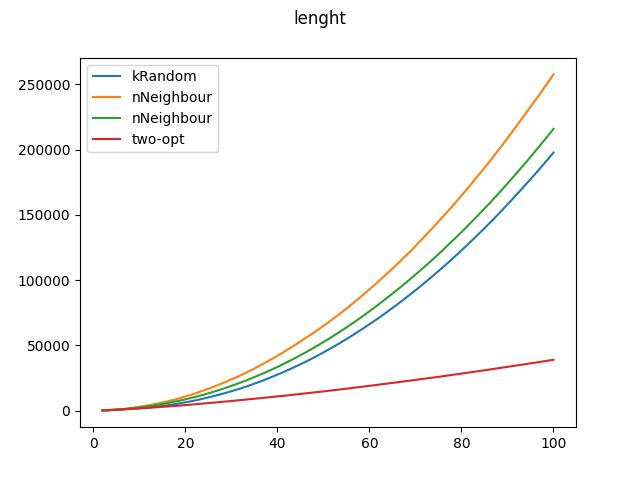
\includegraphics[scale=0.7]{images/lenght_sym.png}\

            \end{figure}
            \end{center}
            \begin{center}
            \begin{figure}[H]

                \\ 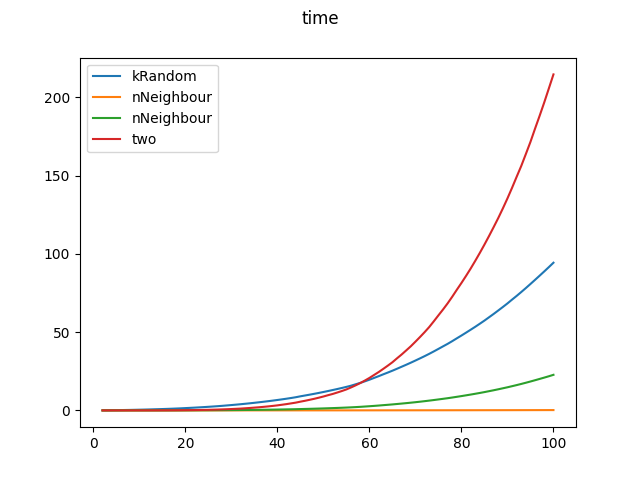
\includegraphics[scale=0.7]{images/time_sym.png}\

            \end{figure}
            \end{center}
\subsubsection{Instancja Asymetryczna }
            \begin{center}
            \begin{figure}[H]

                \\ 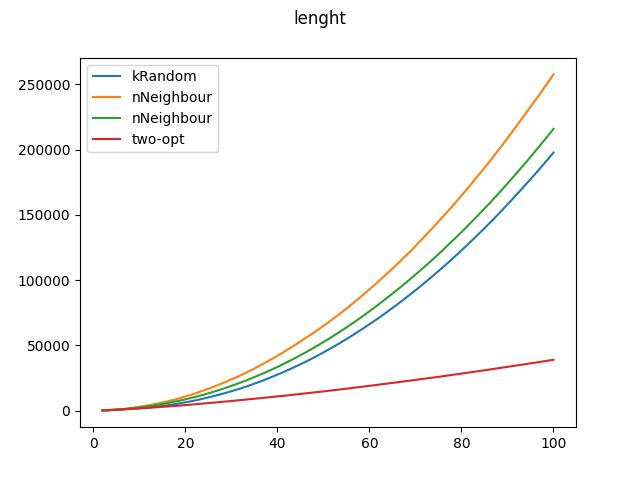
\includegraphics[scale=0.7]{images/lenght_sym.png}\

            \end{figure}
            \end{center}
            \begin{center}
            \begin{figure}[H]

                \\ 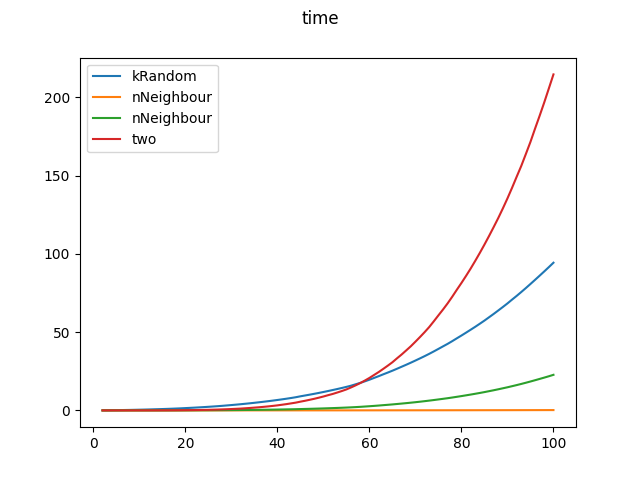
\includegraphics[scale=0.7]{images/time_sym.png}\

            \end{figure}
            \end{center}
\subsubsection{Instancja Euklidesowa }
            \begin{center}
            \begin{figure}[H]

                \\ 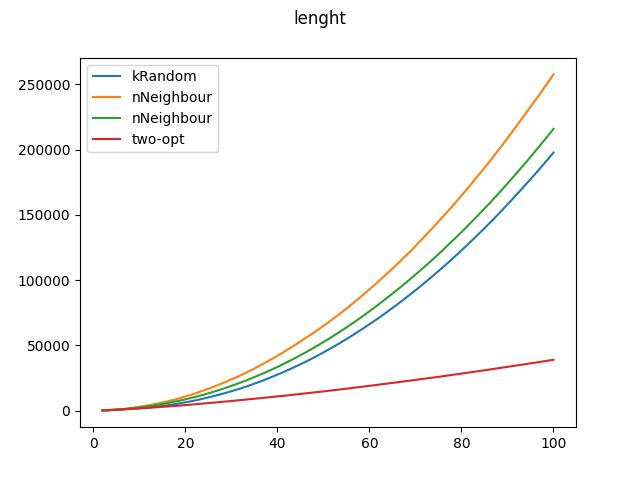
\includegraphics[scale=0.7]{images/lenght_sym.png}\

            \end{figure}
            \end{center}
            \begin{center}
            \begin{figure}[H]

                \\ 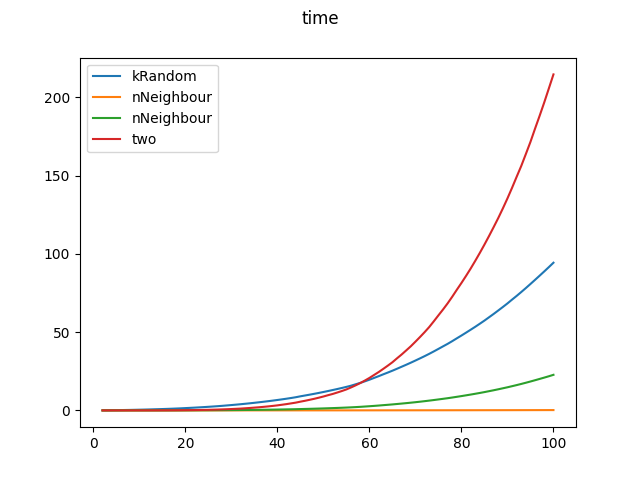
\includegraphics[scale=0.7]{images/time_sym.png}\

            \end{figure}
            \end{center}
\subsection{Wnioski }   
Z wykresów wynika jasno przewaga rozwiązań zwróconych przez algorytm two-opt. Warto zauważyć również że najszybszym algorytmem jest algorytm najbliższego sąsiada, a najwolniejszym two-opt. Jeśli zależy nam na jakości rozwiązań a nie na czasie two-opt jest najlepszy wśród badanych. 
\section{Jakość rozwiązań w tym samym czasie }
\\W poprzednim punkcie algorytm two-opt zwracał najlepsze wyniki ale najwolniej, dlatego aktualnie badanie zostanie przeprowadzone dla czasu $t$, takiego samego dla każdego algorytmu. Ponieważ można łatwo sterować czasem wykonywania algorytmów k-random oraz two-opt, $t$ będzie równe czase, wykonywania rozszerzonego algorytmu najbliższego sąsiada a jego końcem.
\subsection{Wykresy }
\subsubsection{Instancja Symetryczna }
            \begin{center}
            \begin{figure}[H]

                \\ 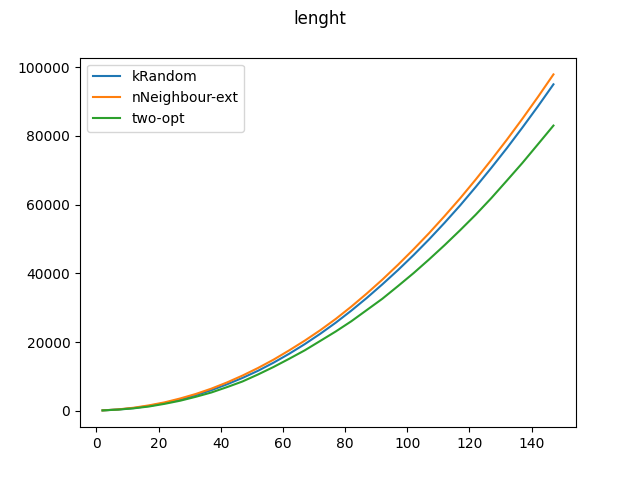
\includegraphics[scale=0.6]{images/lenght_sym_time.png}\

            \end{figure}
            \end{center}

\subsubsection{Instancja Asymetryczna }
            \begin{center}
            \begin{figure}[H]

                \\ 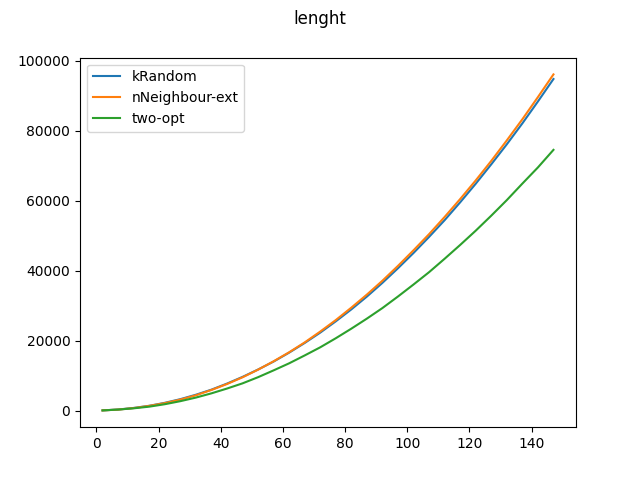
\includegraphics[scale=0.6]{images/lenght_asym_time.png}\

            \end{figure}
            \end{center}
\subsubsection{Instancja Euklidesowa }
            \begin{center}
            \begin{figure}[H]

                \\ 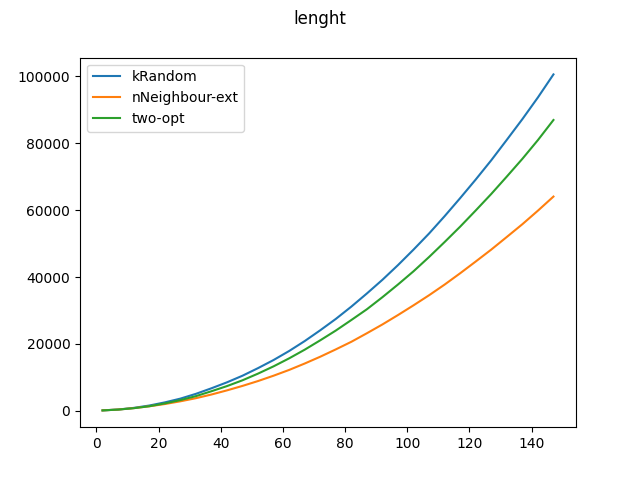
\includegraphics[scale=0.6]{images/lenght_euc_time.png}\

            \end{figure}
            \end{center}
\subsection{Wnioski }
W instancach symetrycznych oraz asymetrycznych znowu wygrywa two-opt, teraz jednak czas wynonywania wynosi jest równy, pozostałe algorytmy są do siebie zbliżone. Natomiast w instancji Euklidesowej najlepszym okazuję się rozszerzony algorytm najbliższego sąsiada.
\end{document} 